\documentclass[a4paper,12pt]{article}
\usepackage[utf8]{inputenc}
\usepackage[russian,english]{babel}
\usepackage[breaklinks=true]{hyperref}
\usepackage{url}
\usepackage{geometry}
\geometry{top=2cm, bottom=2cm, left=2.5cm, right=2.5cm}
\usepackage{titlesec}
\usepackage{fancyhdr}
\usepackage{enumitem}
\usepackage{amsmath}
\usepackage{graphicx}
\usepackage{float} 
\usepackage{listings}
\usepackage{verbatim}
\usepackage{fvextra}

\titleformat{\section}{\Large\bfseries}{\thesection}{1em}{}
\titleformat{\subsection}{\large\bfseries}{\thesubsection}{1em}{}

\pagestyle{fancy}
\fancyhf{}
\fancyhead[L]{Simplified Gossip Protocol}
\fancyhead[R]{Project Report}
\fancyfoot[C]{\thepage}

\begin{document}

\begin{titlepage}
    \centering
    {\Large \textbf{Simplified Gossip Protocol}}\\[1cm]
    \textbf{Project Report}\\[0.5cm]
    \vfill
    \textbf{Student Names: Arina Zimina, Karina Siniatullina,} \\[0.3cm]
    \textbf{Adelina Karavaeva, Egor Agapov} \\[0.5cm]
    \textbf{Date: 30.04.2025} \\[2cm]
    \vfill
\end{titlepage}

\section{Introduction}

The \textbf{Gossip protocol} is a protocol that allows designing highly efficient, secure and low latency distributed communication systems (P2P). The inspiration for its design has been taken from studies on epidemic expansion and algorithms resulting from it. \\\\
The gossip protocol is very important in distributed systems because it helps \textbf{nodes} (computers, servers, or processes) \textbf{share information quickly}, \textbf{reliably}, and \textbf{without a central coordinator}. Here's why it's critical:
\begin{itemize}
    \item \textbf{Scalability:} Gossip scales really well — even with thousands of nodes — because each node only talks to a few others at a time.
    \item \textbf{Fault tolerance:} Nodes can fail or go offline, but gossip ensures the system can still spread information without depending on any single point.
    \item \textbf{Eventually consistent:} Perfect synchronization is hard in distributed systems, so gossip allows nodes to eventually reach the same state without requiring immediate consistency.
    \item \textbf{Low overhead:} The communication is lightweight and randomized, so it doesn't overload the network.
\end{itemize}

\textbf{A few important use cases for gossip protocols:}
\begin{enumerate}
    \item \textbf{Membership tracking:} Nodes use gossip to find out which other nodes are alive, dead, or new in the system (example: Amazon DynamoDB).
    \item \textbf{State dissemination:} Systems like Apache Cassandra use gossip to spread metadata (like schema changes, load info) across all nodes.
    \item \textbf{Failure detection:} If a node crashes, gossip helps quickly alert the rest of the system so they can reroute traffic or rebalance data.
    \item \textbf{Blockchain and cryptocurrency networks:} In Bitcoin, Ethereum, and other decentralized networks, gossip spreads new transactions and blocks across peers.
\end{enumerate}

\section{Methods}

Our implementation of the Gossip Protocol consists of a modern web application with a clear separation between backend and frontend components. The system architecture is designed to be scalable, maintainable, and provides real-time visualization of the gossip protocol simulation.

\subsection{Architecture}
The project follows a client-server architecture:
\begin{itemize}
    \item \textbf{Backend:} Implemented in Python using FastAPI framework, providing RESTful API endpoints for simulation control and data retrieval
    \item \textbf{Frontend:} Built with React.js, offering a modern, interactive user interface with:
        \begin{itemize}
            \item Real-time visualization of node states and message propagation
            \item Interactive controls for simulation parameters
            \item Animated transitions using Framer Motion for smooth node state changes
            \item Responsive design for various screen sizes
        \end{itemize}
    \item \textbf{Communication:} REST API with CORS support for seamless frontend-backend interaction
\end{itemize}

\subsection{Simulation Implementation}
The core simulation logic is implemented in the following components:
\begin{itemize}
    \item \textbf{Node Class:} Represents individual nodes in the network with properties for:
        \begin{itemize}
            \item Node identification
            \item Data storage
            \item Active/inactive states
            \item Alive/dead states
        \end{itemize}
    \item \textbf{Gossip Algorithm:} Implements the core protocol with features:
        \begin{itemize}
            \item Random peer selection
            \item Concurrent message exchange using threading
            \item Fault tolerance simulation (1\% node failure probability)
            \item Node recovery simulation (5\% recovery probability)
            \item Convergence detection
        \end{itemize}
\end{itemize}

\subsection{Convergence and Metrics}
The system tracks several important metrics:
\begin{itemize}
    \item \textbf{Convergence:} Detected when all alive nodes have the same data
    \item \textbf{Round History:} Each round's state is saved, including:
        \begin{itemize}
            \item Node states (active/inactive, alive/dead)
            \item Flagging whether the message has reached the node
            \item Message exchanges
            \item Convergence status
        \end{itemize}
    \item \textbf{Simulation Logs:} Detailed JSON logs for each simulation round
\end{itemize}

\subsection{Tools and Technologies}
\begin{itemize}
    \item \textbf{Backend:} Python, FastAPI, threading
    \item \textbf{Frontend:} 
        \begin{itemize}
            \item React.js for component-based UI development
            \item Framer Motion for smooth animations and transitions
            \item Modern CSS for responsive design
            \item WebSocket for real-time updates
        \end{itemize}
    \item \textbf{Development:} Git for version control
    \item \textbf{Testing:} Dedicated test suite for protocol verification
\end{itemize}

\section{Results}

\subsection{Interface}
The initial interface of the algorithm looks simple and straightforward and allows you to select the number of nodes, the message to be exchanged and the node id of the node from which the algorithm will start executing.
\begin{figure}[H]
    \centering
    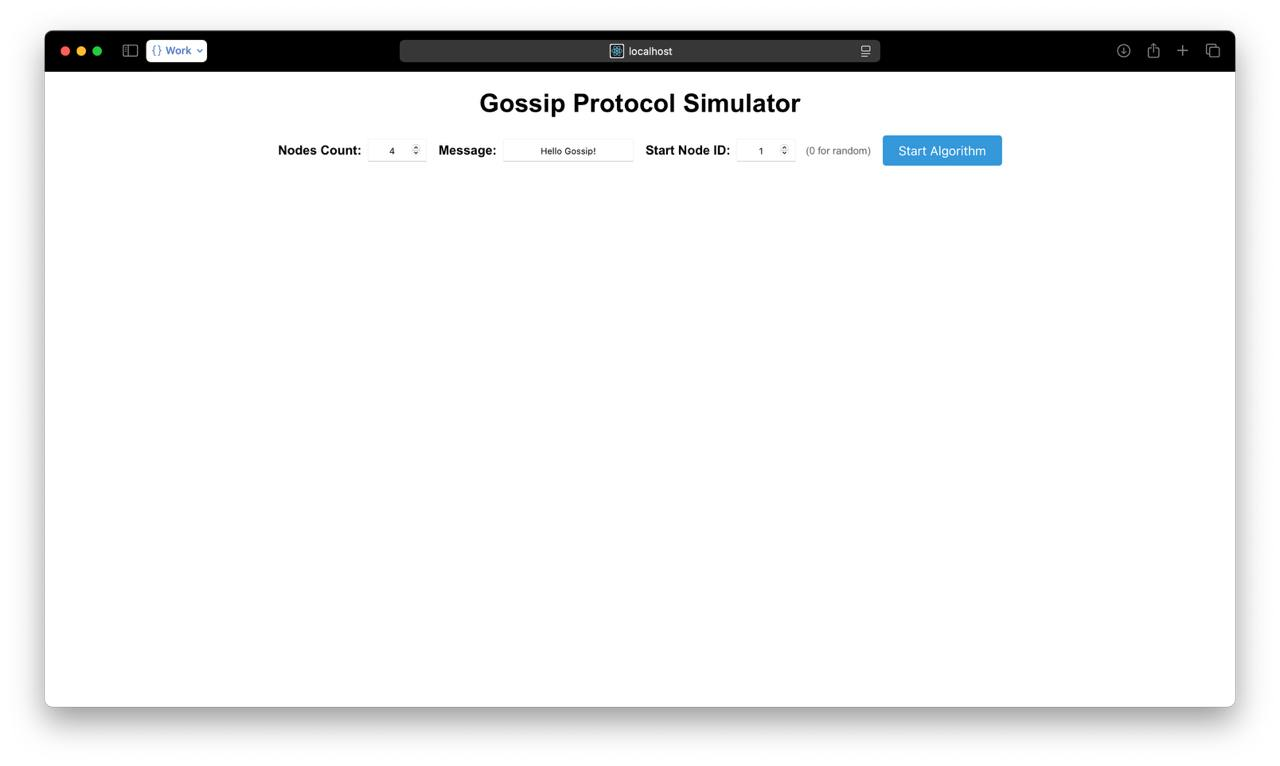
\includegraphics[width=0.8\textwidth]{figures/interface.jpeg}
    \label{fig:screenshot1}
\end{figure}

\subsection{Algorithm visualization}
At each round, the visualization shows the state of each node, the process of message exchange between specific nodes and the round number. If a message reaches a particular node, a green checkmark is displayed on the corresponding monitor.
\begin{figure}[H]
    \centering
    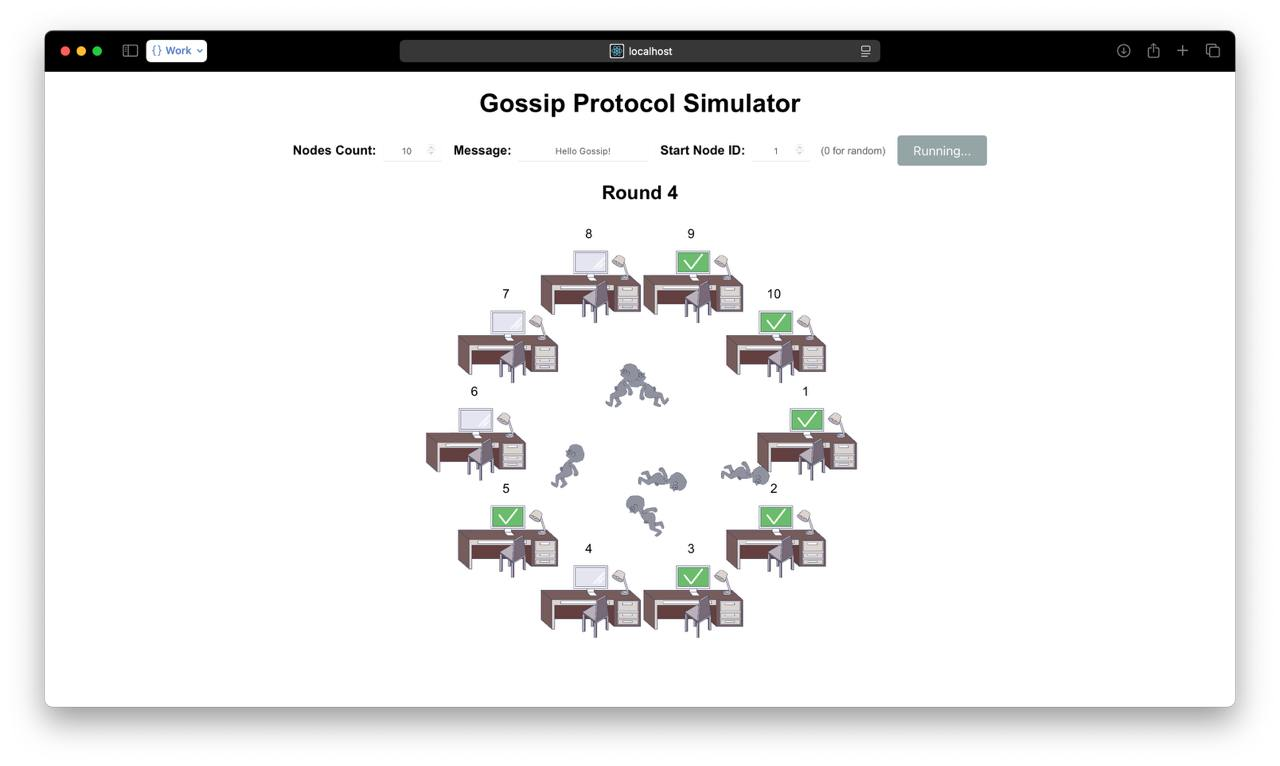
\includegraphics[width=0.8\textwidth]{figures/alg_visualisation.jpeg}
    \label{fig:screenshot3}
\end{figure}

The completion of the algorithm looks like this:
\begin{figure}[H]
    \centering
    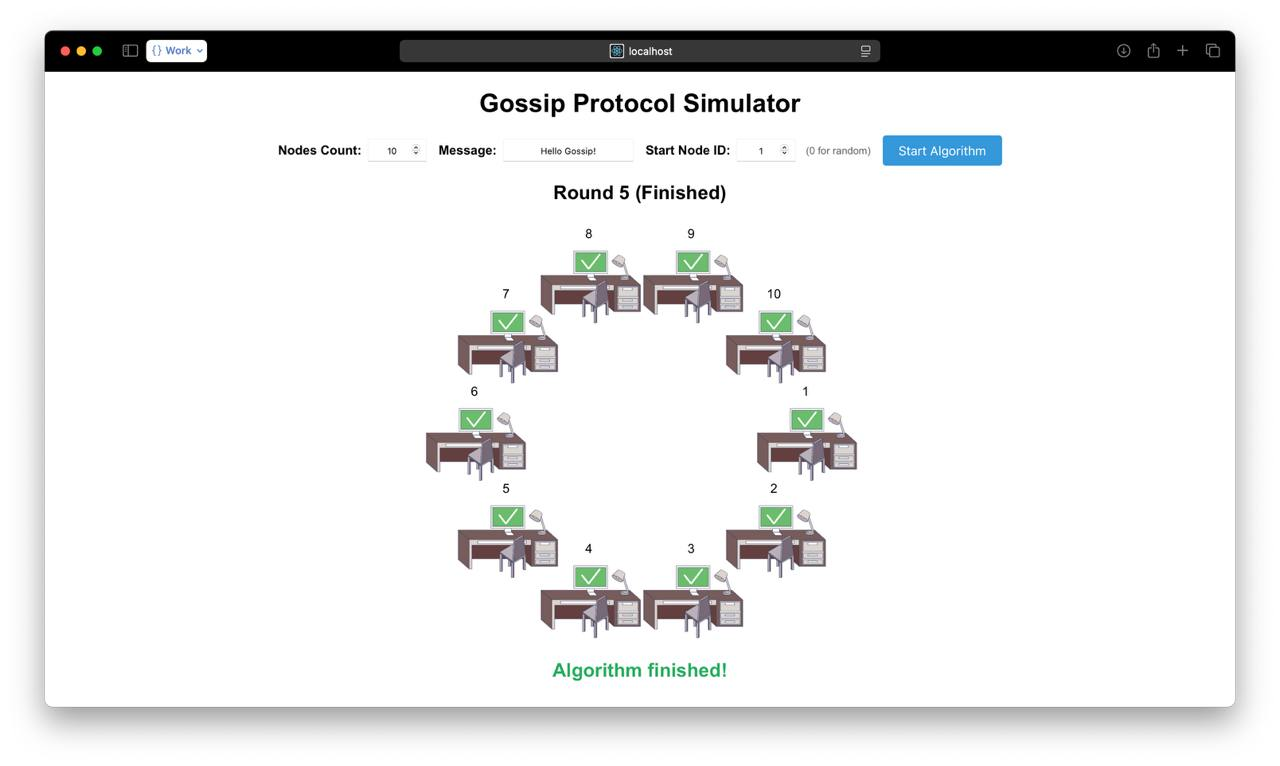
\includegraphics[width=0.8\textwidth]{figures/finished.jpeg}
    \label{fig:screenshot4}
\end{figure}

A dead node during the algorithm process is marked with a red screen with a skull on it:
\begin{figure}[H]
    \centering
    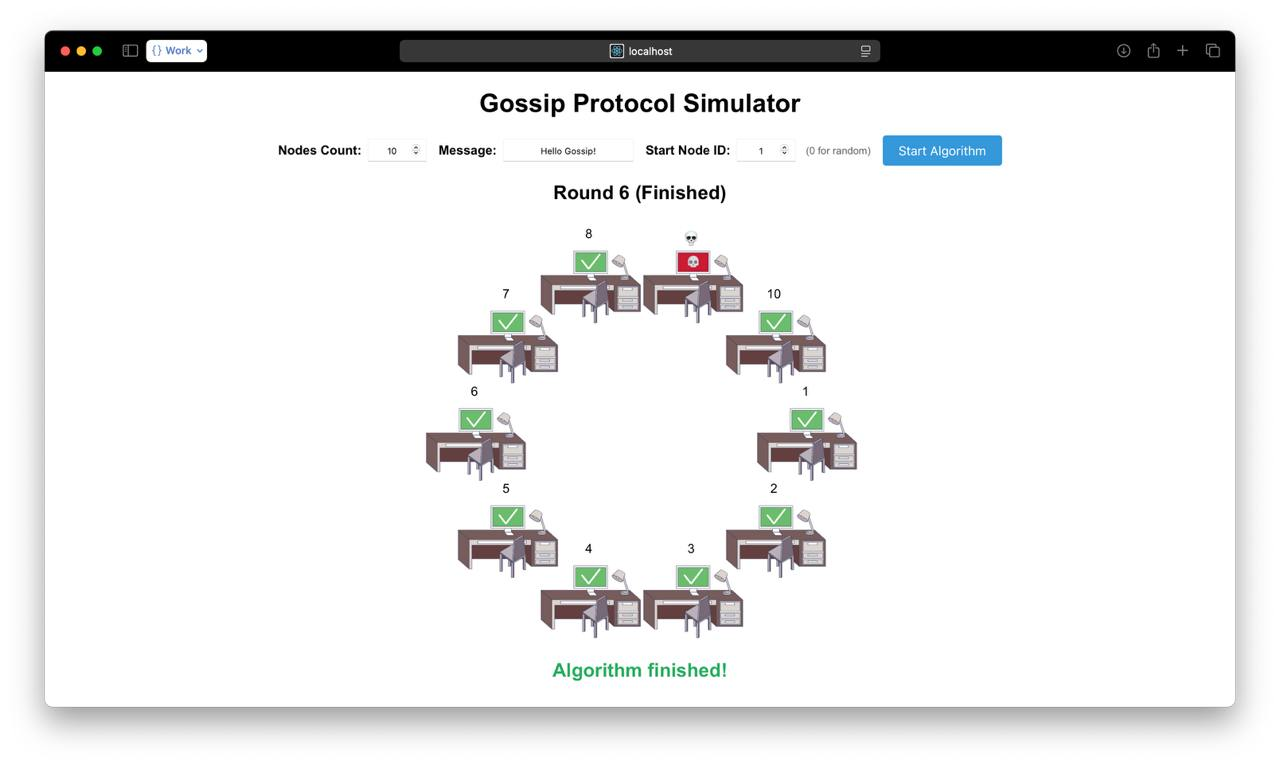
\includegraphics[width=0.8\textwidth]{figures/node_dead.jpeg}
    \label{fig:screenshot5}
\end{figure}

\subsection{Logs}
Our logs are collected every round. At the beginning we write the number of the round, then a checkbox whether the exchange of information has been completed (final round), then a description of the state of each node in the algorithm and then a list of messages exchanged by the nodes in this round. 
\begin{figure}[H]
    \centering
    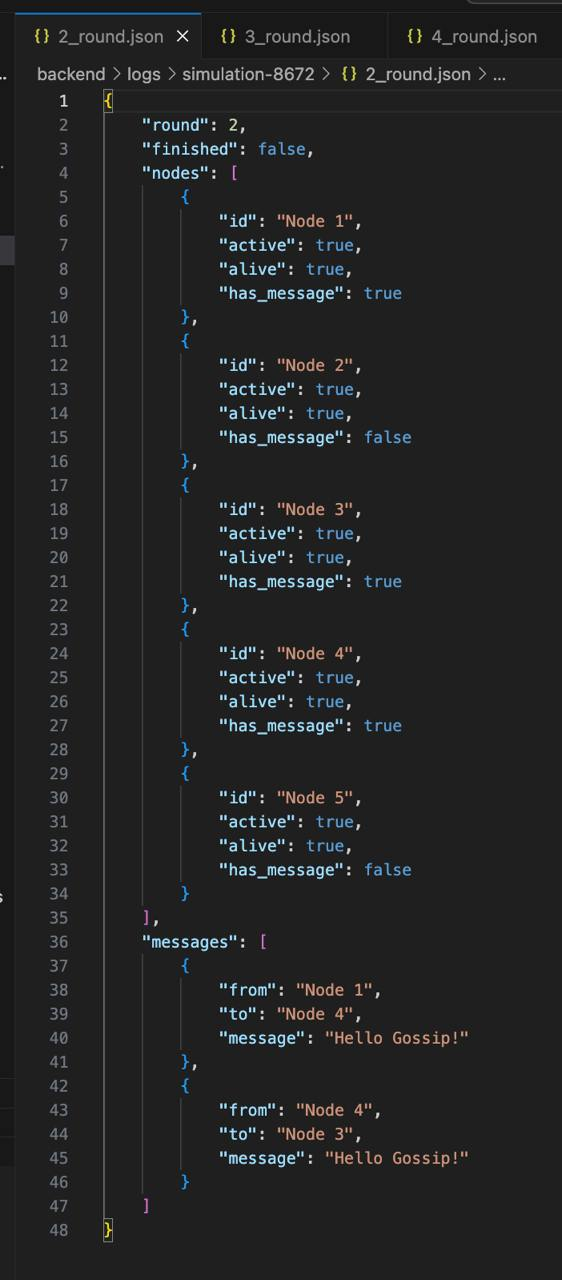
\includegraphics[width=0.5\textwidth]{figures/logs.jpg}
    \label{fig:screenshot2}
\end{figure}

\section{Discussion}

\subsection{What has been achieved}
\begin{itemize}
    \item The basic logic of the algorithm is fully implemented
    \item The ability to select the number of nodes in the algorithm has been implemented
    \item The visuals on the web page are hand-drawn
    \item At the end of each round, comprehensible logs are generated
    \item A simple and clear web page design and interface has been implemented
    \item Possibility to enter the message exchanged between nodes in the algorithm
    \item Added the ability to select the node id of the node from which we start executing the algorithm
\end{itemize}

\subsection{What has not been achieved}
\begin{itemize}
    \item We have not been able to deal with the comprehensibility and accessibility of the web interface for a large number of nodes (e.g. starting from 100)
    \item It was not possible for us to implement data transmission simulating real network delays
\end{itemize}
Despite these limitations, the core functionality of the project works reliably, and the simulation successfully demonstrates the intended behavior of the gossip protocol. The project serves as a solid foundation for further improvements and scaling.

\subsection{What could be improved}
\begin{itemize}
    \item \textbf{Scalability:} The current implementation could be optimized to better handle simulations involving hundreds or thousands of nodes, both in terms of performance and UI clarity.
    \item \textbf{Realism:} Introducing configurable network delays and message loss rates would make the simulation more realistic and useful for testing fault tolerance.
    \item \textbf{Number of messages:} Add the ability to send multiple messages from different nodes as well as the ability to select the number of messages a node can send per round.
\end{itemize}

\section{References}

\begin{enumerate}
    \item What is the Gossip Protocol: \url{https://academy.bit2me.com/en/what-is-gossip-protocol/}
    \item To visualize people in the algorithm: \url{https://codepen.io/MAW/full/RaXRdE/}
    \item Gossip Protocol: \url{https://en.wikipedia.org/wiki/Gossip_protocol}
    \item Gossip Protocol implementation: \url{https://hyperledger-fabric.readthedocs.io/ru/latest/gossip.html}
    \item The basic idea behind the Gossip Protocol: \url{https://neerc.ifmo.ru/wiki/index.php?title=Gossip-протоколы}
    \item FastAPI Documentation: \url{https://fastapi.tiangolo.com}
    \item React Documentation: \url{https://react.dev}
    \item CSS Animations: \url{https://developer.mozilla.org/en-US/docs/Web/CSS/CSS_animations/Using_CSS_animations}
    \item Motion Animation Library: \url{https://motion.dev}
\end{enumerate}
\end{document}